\documentclass[12pt]{article}

\usepackage[brazil,american]{babel}
\usepackage[utf8]{inputenc}
\usepackage[a4paper, total={6.5in, 9.5in}]{geometry}

\usepackage{url}
\usepackage{graphicx}
\usepackage{authblk}
\usepackage{hyperref}
\usepackage{lipsum}
\usepackage{xcolor}
\usepackage{float}
\usepackage{listings}

\definecolor{codegreen}{rgb}{0,0.6,0}
\definecolor{codegray}{rgb}{0.5,0.5,0.5}
\definecolor{codered}{rgb}{0.8,0,0}
\definecolor{backcolour}{rgb}{0.95,0.95,0.92}

\usepackage{inconsolata}
\lstset{
    language=python,
    % backgroundcolor=\color{backcolour},   
    commentstyle=\color{codegreen},
    keywordstyle=\color{blue},
    numberstyle=\tiny\color{codegray},
    stringstyle=\color{codered},
    basicstyle=\ttfamily\small,
    % numberstyle=\footnotesize,
    % numbers=left,
    % backgroundcolor=\color{gray!10},
    % frame=single,
    tabsize=2,
    rulecolor=\color{black!30},
    title=\lstname,
    escapeinside={\%*}{*)},
    breaklines=true,
    breakatwhitespace=true,
    framextopmargin=2pt,
    framexbottommargin=2pt,
    inputencoding=utf8,
    extendedchars=true,
    showstringspaces=false,
    literate={á}{{\'a}}1 {ã}{{\~a}}1 {é}{{\'e}}1 {Ó}{{\'O}}1 {Ã}{{\~A}}1 {í}{{\'i}}1 {ó}{{\'o}}1,
}

% \pagecolor[rgb]{0.1,0.1,0.1}
% \color[rgb]{0.9,0.9,0.9}

\begin{titlepage}
    \title{
        
\includegraphics[width=4cm]{img/logo.jpg} \\ 
        \large
        Dep. Ciência da Computação -- Universidade de Brasília (UnB)\\
        CIC0124 - Redes de Computadores, Turma A \\
        \vfill 
        \vfill
        \LARGE
        \textbf{Projeto Final\\
        Cliente DASH}
        \vfill
    }

    \author{
        Kesley Kenny Vasques Guimarães, 18/0021231\\
        Pedro Henrique de Brito Agnes, 18/0026305\\
        Victor Alves de Carvalho, 16/0147140
    }
    
    \affil{
        \vfill
        \vfill
        \vfill
        Professor \\
        Dr. Marcos Fagundes Caetano
    }

    \date{Brasília\\Dezembro de 2020}

\end{titlepage}

\begin{document}
\maketitle
\newpage

\selectlanguage{brazil}

\section{Introdução}
Para a implementação de um cliente DASH, existem diversos fatores a considerar. A largura de banda disponível aos usuários pode ser instável no geral, o que dificulta um serviço de \textit{streaming} de vídeo estável, ou seja, sem pausas ou de qualidade. Por isso, os serviços desse tipo atualmente disponibilizam diversas qualidades da imagem do vídeo diferentes, onde é atribuída a qualidade ideal, com o tempo necessário para baixar mais adequado à realidade da internet do usuário.


Outro conceito utilizado é o de \textit{buffer}, que é um local onde serão armazenados os segmentos de vídeo baixados para a reprodução ao usuário posteriormente. De maneira geral, os segmentos a serem reproduzidos ao usuário vêm do \textit{buffer}, que é útil para as flutuações de banda, onde no caso de o usuário experienciar uma queda na qualidade da internet, naturalmente vai demorar mais para obter um segmento de uma qualidade melhor, o que pode diminuir o tamanho do \textit{buffer}, mas são usados métodos para evitar ao máximo que o tamanho do mesmo chegue em 0, que resultaria em uma pausa indesejada no vídeo. Para o controle de todos os fatores variáveis incluídos em um cliente DASH, são usados Algoritmos de Adaptação de Taxa de Bits (ABR).

\subsection{Como são implementados os algoritmos ABR?}
Algoritmos ABR são implementados por meio de um balanceador disposto a equilibrar o desempenho da internet do usuário, bem como, a qualidade de reprodução de um provedor de serviços de streaming. O balanceador consiste em algoritmos que devem avaliar os recursos e estatísticas disponíveis de forma a buscar a melhor experiência ao usuário que está usando o serviço de vídeo. Além disso, deve lidar com diferentes tipos de conexão de internet, diferentes tipos de dispositivos de streaming e cálculos de estimativa da bandalarga utilizada.

\subsection{Design ABR}
De modo geral, algoritmos ABR devem ser capazes de atender as seguintes especificações:
\begin{itemize}
    \item \textbf{Maximizar eficiência:} aplicar a melhor taxa de bits durante a exibição de players de vídeo.
    \item \textbf{Minimizar rebuffering:} fazer o possível para que a bandalarga não seja inferior a necessária para a renderização do vídeo.
    \item \textbf{Estabilizar a qualidade do vídeo:} balancear, de modo a não gerar oscilações relacionadas a qualidade do vídeo.
    \item \textbf{Qualidades justas de transmissão:} não pode haver desperdício dos recursos disponíveis. Deve tirar o melhor proveito que a conexão fornece ao usuário.
\end{itemize}

\subsection{Algoritmo aplicado}
Para o projeto, o algoritmo utilizado foi baseado em conceitos obtidos por meio de estudos de algoritmos ABR distintos. Entretanto, nenhum algoritmo específico foi utilizado. A abordagem principal foi seguir todos conceitos de design ABR na tentativa de obter os melhores resultados.



\newpage

\section{Algoritmo ABR}
Para a solução do problema, foi implementado um algoritmo de adaptação de taxa de bits para tentar entregar a melhor qualidade ao usuário com base na banda disponível evitando ao máximo pausas indesejadas no vídeo. Para começar, foram seguidos alguns conceitos básicos, para calcular a qualidade máxima possível de baixar sem perdas com base no \textit{throughtput}, como podemos ver abaixo o método usado para tal:

\begin{lstlisting}
# Maior qualidade com base na taxa de bits sem recorrer ao buffer
def calcula_qualidade_maxima(self, throughput):
    qualidade_index = 0
    for i in range(len(self.qi)):
        qualidade = self.qi[i]
        if throughput < qualidade:
            if i == 0:
                qualidade_index = 0
            else:
                qualidade_index = i-1
            break
        elif i == len(self.qi)-1:
            qualidade_index = len(self.qi)-1

    return qualidade_index
\end{lstlisting}

Usando apenas o código apresentado acima é uma forma de se obter uma qualidade ideal para a banda disponível, mas existem alguns problemas que serão listados a seguir. Só é possível calcular a velocidade da internet após a requisição, durante a resposta, o que tem péssimas consequências em redes instáveis, pois se a banda piora, a qualidade selecionada do vídeo ainda continua a mesma e isso quer dizer que vai demorar mais tempo para baixar, o que trará consequências no \textit{buffer}, que será utilizado para que não hajam pausas no vídeo. Assim chegamos no segundo problema da abordagem, que o buffer nunca ficará com um tamanho estável, já que estamos sempre pegando a maior qualidade suportada pelo \textit{throughput}, o que fará com que ele nunca seja suficiente para as quedas de qualidade de internet.

Devido ao problema mostrado acima, foi definida uma forma de calcular um \textit{buffer estável}, que representará o tamanho do \textit{buffer} mínimo para que não existam pausas no vídeo caso a qualidade da rede do usuário caia um tanto considerável. De forma geral, é o tamanho que vai suprir o tempo médio necessário para baixar um segmento na qualidade atual com a pior taxa de internet já registrada durante a execução.

\begin{lstlisting}
# limitar a qualidade escolhida com base no tamanho do buffer
def limite_porcento_qualidade(self, qualidade):
    stable_buffer = self.qi[qualidade]/self.menor_taxa
    stable_buffer += 5 # garantia de seguranca

    limite = self.current_buffer/stable_buffer
    if limite > 1:
        limite = 1

    return limite
\end{lstlisting}

Apesar de todas as verificações, a estratégia ainda se mostra insuficiente, pois utiliza como base a pior taxa de transferência já registrada, o que não será muito útil se a qualidade da rede começar boa no início do vídeo e cair depois. Para isso, foi implementada uma função que vai priorizar o carregamento do \textit{buffer} ao início da reprodução do vídeo, limitando a qualidade proporcionalmente ao tempo passado seguindo uma função logarítmica. O funcionamento da mesma é de forma que a qualidade do vídeo vai seguir o comportamento da função definida no gráfico até atingir a qualidade suportada máxima pelo \textit{throughput}, assim garantindo um tempo bom para o carregamento inicial do \textit{buffer}. Podemos ver o comportamento a seguir:

\begin{figure}[H]
    \centering
    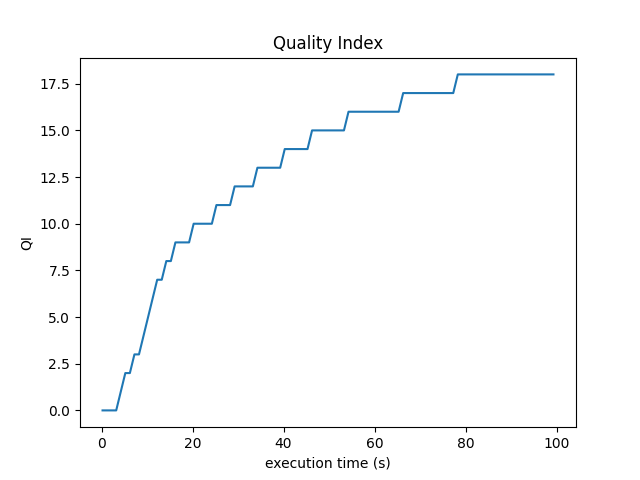
\includegraphics[width=.75\textwidth]{img/qi_L.png}
    \caption{Sequência L com a função logarítmica}
\end{figure}

Por fim, também foi criado um método para controlar as quedas de qualidade de forma a não cair de uma vez para zero, que prejudica e experiência do usuário e, portanto, vai diminuir de pouco a pouco até chegar na pior qualidade. A seguir será mostrado o método que basicamente conta as quedas consecutivas de \textit{throughput} e corrige a qualidade com base nela para valores médios entre a média geral, 0 e a qualidade atual.

\begin{lstlisting}
# impede a qualidade de cair imediatamente com condicoes especificas
def suavisa_queda_qualidade(self, qualidade):
    self.quedas_consecutivas += 1
    qualidade_corrigida = 0

    qualidade_atual = 0
    for q in self.qi:
        if q == self.current_quality:
            break
        qualidade_atual += 1

    media = self.avg_qi()

    if self.quedas_consecutivas == 1:
        qualidade_corrigida = (qualidade_atual + media)/2
    elif self.quedas_consecutivas == 2:
        qualidade_corrigida = media
    elif self.quedas_consecutivas == 3:
        qualidade_corrigida = media/2

    return math.floor(qualidade_corrigida)
\end{lstlisting}

Com todas essas especificações, obtemos o nosso ABR final é quase igualmente otimizado em relação às pausas e à qualidade. Além disso, o algoritmo roda de forma bem constante, entregando a melhor qualidade possível com a banda, porém de forma \textit{segura}, para evitar as pausas ao máximo, balanceando entre os dois fatores.

\section{Conclusões}
O trabalho ajudou-nos a entender melhor sobre o funcionamento dos serviços de \textit{streaming}, que dominam a internet na atualidade, assim como mostrando diversas dificuldades na implementação. Durante o desenvolvimento do projeto, foi necessário escolher entre priorizar a qualidade ou as pausas, onde foi feito o possível para atender aos dois.

\begin{thebibliography}{9}

\bibitem{livroRC}
\noindent James F. Kurose \& Keith W. Ross, 
\textit{Redes de Computadores e a Internet - Uma nova Abordagem, 7a /8a Edição, Pearson Education / Makron Books.}

\bibitem{video}
\noindent Streaming Media Editorial Staff.
\textit{Why Adaptive Bitrate Streaming?}, 2016

\bibitem{artigo1}
\noindent Iraj Sodagar.
\textit{The MPEG-DASH Standard for Multimedia Streaming Over the Internet}

\end{thebibliography}

\end{document}
